\chapter[Documento de Visão]{Documento de Visão}

\section{Introdução}
A finalidade deste documento é coletar, analisar e definir necessidades e recursos de nível superior do <<Nome do Sistema>>. Ele se concentra nos recursos necessários aos envolvidos e aos usuários-alvo e nas razões que levam a essas necessidades. Os detalhes de como o <<Nome do Sistema>> satisfaz essas necessidades são descritos nas especificações de requisitos.

\subsection{Finalidade}
Este documento tem a finalide de  esclarecer e possibilitar uma visão do sistema que será uma informação importante para o entendimentos dos envolvidos no projeto.
\subsection{Escopo}
Este está inserido em um contexto de especificação dos usuários que estarão utilizando o sistema, os interessados no projeto, os requisitos não funcionais, sistemas semelhantes, recursos e características. Bem como a indicação da documentação que será desenvolvida para auxílio dos usuários ao utilizar o sistema.
\subsection{Visão Geral}
Este documento está dividido em doze sessões, descrevendo o Posiconamento do Projeto, Usuários, Visão Geral do Produto, Recursos do Produto, Restrições, Intervalos de Qualidade, Outros Requisitos do Produto, Requisitos de Documentação, Análise dos Softwares Semelhantes, Desenvolver, Comprar ou Customizar? e por fim, Subsistemas que o <<Nome do Sistema>> possui.

\section{Posicionamento}

\subsection{Oportunidade de Negócios}
Dado o grande numero de acidentes que ocorrem no Brasil, percebe-se que com o
desenvolvimento de um sistema de alerta na ultrapassagem, pode-se obter
ganhos ao evitar gastos com as consequências dos acidentes para todos os
brasileiros usuários das rodovias. Dado que, segundo a PRF, o tipo de acidente
que mais mata é a colisão frontal, causada, especialmente, pelas ultrapassagens
forçadas ou em locais sem visibilidade\cite{prf}.

\subsection{Descrição do Problema}
\begin{table}[ht]
\caption{Framework do Problema}
\centering
\begin{tabular}{| l |  p{7cm} |}
\hline
O problema da & Grande quantidade de acidentes, cuminando em mortes, que acontecem nas rodovias brasileiras devido a execução de ultrapassagens.  \\
\hline
Afeta & O povo brasileiro que é usuário das rodovias como meio de transporte. \\
\hline
Cujo o impacto é & A Morte de vários brasileiros, bem como a perca de bens materiais no momento do acidente.\\
\hline
Uma boa solucao seria & A Implementação de um sistema que possibilite a sinalização ao motorista sobre quando e possivel executar a ultrapassagem. \\
\hline
\end{tabular}
\end{table}


\subsection{Sentença de Posição do Produto}

\begin{table}[ht]
\caption{Designação do Produto}
\centering
\begin{tabular}{| l |  p{7cm} |}
\hline
Para & Brasileiros que utilizam as rodovias como meio de locomoção a partir de qualquer automóvel. \\
\hline
Que & Evitará os acidentes no momento que os usuários das rodovias forem executar ultrapassagens. \\
\hline
O <<Nome do produto>> & É uma categoria de sistenas de segurança\\
\hline
Que & Culminará na queda dos indicares de mortalidade devido a acidentes de transito nas rodovias decorrentes de ultrapassagens \\
\hline
Diferente de & Produtos pré instalados em carros adquiridos em concenssonárias e que não são fornecidos no Brasil.  \\
\hline
Nosso Produto & Pode ser adiquirido por qualquer motorista para qualquer automóvel no Brasil\\
\hline
\end{tabular}
\end{table}


\section{Descrições dos Envolvidos e dos Usuários}

\subsection{Perfil dos Usuários}
O perfil do público alvo desejado pelos integrantes do projeto é o de qualquer cidadão que possua carteira de motorista reconhecida em território nacional, de acordo com o Código de Trânsito Brasileiro\cite{ctb}.

\subsection{Ambiente do Usuário}
O ambiente de uso do sistema será as rodovias brasileiras. O sistema estará instalado no carro do usuário e emitirá os devidos alertas ao mesmo de acordo com as especificações que serão abordadas neste relatório.

\subsection{Perfil dos Envolvidos}
Os envolvidos na elaboração/idealização técnica do produto são os alunos graduandos da Universidade de Brasília - Faculdade do Gama cursando a disciplina de Projeto Integrador.

\section{Recursos do Produto}
Os tópicos a seguir ilustrarão quais as capacidades do nosso sistema.
\subsection{Acionamento da verificação de segurança}
O motorista poderá acionar o sistema de segurança ao ter a intenção de ultrapassar.
Quando este acionar o sistema através de alguma entrada, será executado o algorítimo para a verificação da possibilidade de
ultrapassagem, analisando se o caminho a ser percorrido para ultrapassar está em condições desejávies, isto é,
se não há nenhum outro carro vindo na direção oposta em codição de colisão.

\subsection{Alerta de Perigo}
Ao analisar a possibilidade de ultrapassagem, o sistema irá alertar ao motorista caso esta seja insegura.

\section{Restrições}
Devido a quantidade de acidentes decorridos de ultrapassagens ser maior em rodovias, nosso sistema tera a restriçao de atender apenas os usuarios transitando nestes locais. Alem disso, o trafico de automoveis em todas as direcoes e muito alto, cuminando assim na ineficiencia do sistema ao detectar a todo momento que a ultrapassagem e inadequada.

Dessa maneira, a utilizacao do projeto dentro de cidades nao viavel, possibilitando o uso apenas em rodivias.

\section{Requisitos de Documentação}
Esta seção descreve a documentação que deverá ser desenvolvida para suportar a implantação bem-sucedida de aplicativos.

\subsection{Manual do Usuário}
O sitema contera dentro da embalagem a ser adquirida um manual de instruçoes de uso do sistema, bem como orientaçoes sobre instalacao e manutencao.

\subsection{Ajuda On-line}
Sera disponibilizada uma documentacao online para auxilio do usuario em qualquer aspecto de uso. Serao disponibilizados os manuais fisicos, esta documentacao de desenvolvimento do projeto como: Documento de Visao, Especificaçao dos Requisitos e Prototipos de Tela

\section{Análise dos Softwares Semelhantes}
Recentemente, vários dispositivos anti-colisão têm sido projetados e lançados, entretanto ainda não foi feito um dispositivo com o intuito
de prevenir colisões durante ultrapassagem. A Volvo, por exemplo, desenvolveu um dispositivo de segurança que prevê rotas em situação de
colisão. O sistema possui sensores que permitem monitoramento de 360º ao redor do carro, aprimorado por um gerador de manobra, freio ou controle
automático da direção, um software que identifica possíveis rotas de fuga. Para isso, se fez necessário o desenvolvimento de uma estrutura central
que reúne vários sensores, a fim de permitir que câmeras, radares por ondas, radares por laser e GPS trabalhem em conjunto [1]. A
 Figura \ref{fig:sistemavolvo} ilustra
 o sistema lançado pela empresa.

 \begin{figure}[h]
   \centering

   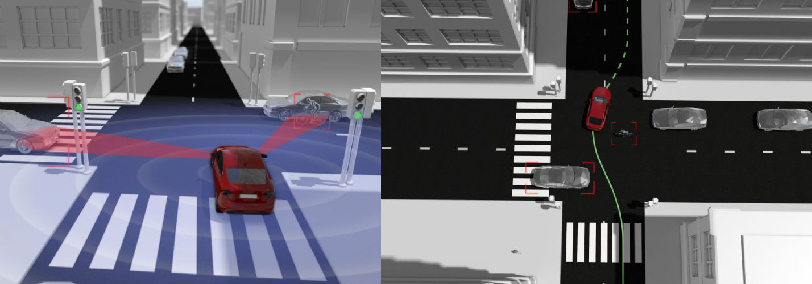
\includegraphics[width=450px, scale=1]{figuras/sistemavolvo}
   \caption{Ilustração do Sistema anti-colisão da Volvo}
\label{fig:sistemavolvo}
 \end{figure}


Outro dispositivo com aplicação semelhante é o da empresa Distritec, que é um sistema anti-colisão que detecta pessoas e objetos, que possui
um sensor de detecção, um display montado na cabine do veículo, tecnologia de radar por pulsos que alerta o usuário quando há algum obstáculo
 parado ou em movimento em uma área pré-definida de 10 metros. O sistema não precisa de limpeza, não é afetado por condições climáticas adversas
  [2].

O dispositivo que foi desenvolvido em um projeto de pesquisa da universidade Mauá, apresenta um sistema de navegação para veículo baseado na
transmissão de dados entre veículos. O sistema utiliza parâmetros estimados para determinar a velocidade e posição relativa de veículos autônomos
e módulos com tecnologia para permitir a comunicação entre veículos e estimar a distância entre os veículos por meio de um algoritmo [3].

Foi feita uma abordagem simples desse tipo de sistema, através de um microcontrolador, um sensor de velocidade e um sensor de distância. O sistema
 pode ser utilizado em vários veículos, com alterações em sua programação, que é feita com liguagem C. O circuito eletrônico é capaz de alertar o
 condutor de um veículo, a qualquer risco eminente de colisão a pouco mais de 6,3 metros, com velocidade máxima de 7 km/h, aproximadamente [4].

A Chevrolet também laçou um sistema anti-colisão, com funcionamento semelhante ao recurso oferecido por outras marcas, porém com apenas uma câmera
 que faz a identificação de eventuais obstáculos à frente, o dispositivo alerta o motorista sobre perigos e freia o veículo automaticamente para
 evitar impactos, assim como o dispositivo lançado pela Volvo, já citado. A General Motors busca popularizar a tecnologia e aplicá-la também nos
 carros mais baratos do portfólio. O sistema é capaz de frear o veículo a velocidades de até 25 km/h [5].

 A Toyota também lançou um modulo de prevenção de colisões, o Pre-Collision System (PCS), que utiliza um sistema de sensores instalados na
 dianteira, que detecta a presença de pedestres, obstáculos ou outros automóveis, radares e câmeras especiais que permitem o cálculo da intensidade
  da frenagem e do movimento da direção necessários para escapar dos perigos da pista. O sistema emite luzes próximas ao infravermelho, com o
  objetivo de melhorar a visibilidade do motorista à noite [6].

 Foi projetado também um sistema constituído de dois alto-falantes localizados próximos a cabeça do motorista e de elementos vibratórios no
 acento, que são acionados por meio de sensores localizados ao redor do carro, o sistema é constituído por dois módulos, o módulo ativação
 identifica a situação de risco e informa ao módulo de alerta, que faz a ativação dos estímulos [7]. A Figura \ref{fig:sistemaanticolisao} ilustra os módulos do sistema.


  \begin{figure}[h]
    \centering
    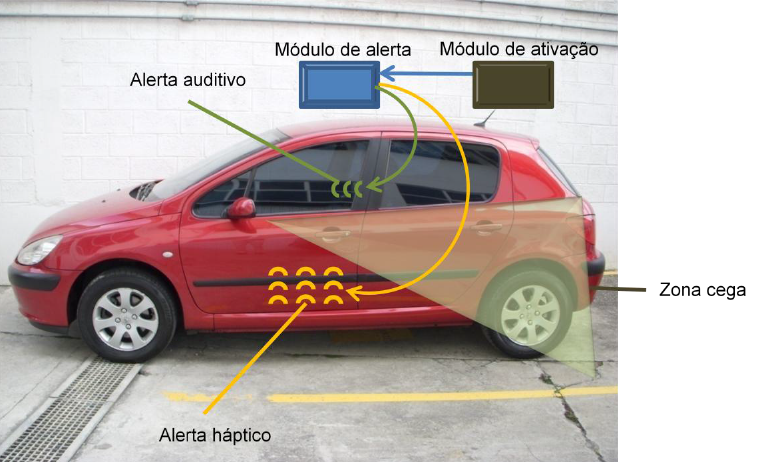
\includegraphics[width=400px, scale=0.5]{figuras/sistemaanticolisao}
    \caption{Esquemático do Sistema anti-colisão}
    \label{fig:sistemaanticolisao}
  \end{figure}


\section{Desenvolver, Comprar ou Customizar?}

\section{Subsistemas}
